\documentclass[a4paper,10pt,preprint,3p,hidelinks]{elsarticle}

\usepackage{lineno}
\modulolinenumbers[5]

\usepackage{booktabs} % added for the table
\usepackage[hidelinks]{hyperref} % removes red boxes around links
\usepackage{placeins}
\usepackage{float}
\usepackage{bm}
\usepackage[latin1]{inputenc}
\usepackage{amsmath}
\usepackage{amsfonts}
\usepackage{amssymb}
\usepackage{graphicx}
\usepackage[textsize=tiny]{todonotes}


\usepackage{color} % add colors for commenting
\newcommand{\tb}[1]{\textbf{#1}}
\newcommand{\bl}[1]{\textcolor[rgb]{0.00,0.00,1.00}{#1}}
\newcommand{\gr}[1]{\textcolor[rgb]{0.00,0.50,0.00}{#1}}
\newcommand{\rd}[1]{\textcolor[rgb]{0.75,0.00,0.00}{#1}}

\usepackage{placeins} % added for \FloatBarrier
%\usepackage[left=1in,right=1in]{geometry}

\journal{ }

%%%%%%%%%%%%%%%%%%%%%%%
%% Elsevier bibliography styles
%%%%%%%%%%%%%%%%%%%%%%%
%% To change the style, put a % in front of the second line of the current style and
%% remove the % from the second line of the style you would like to use.
%%%%%%%%%%%%%%%%%%%%%%%

%% Numbered
%\bibliographystyle{model1-num-names}

%% Numbered without titles
%\bibliographystyle{model1a-num-names}

%% Harvard
%\bibliographystyle{model2-names.bst}\biboptions{authoryear}

%% Vancouver numbered
%\usepackage{numcompress}\bibliographystyle{model3-num-names}

%% Vancouver name/year
%\usepackage{numcompress}\bibliographystyle{model4-names}\biboptions{authoryear}

%% APA style
%\bibliographystyle{model5-names}\biboptions{authoryear}

%% AMA style
%\usepackage{numcompress}\bibliographystyle{model6-num-names}

%% `Elsevier LaTeX' style
\bibliographystyle{elsarticle-num}
%%%%%%%%%%%%%%%%%%%%%%%


\usepackage{blindtext}



\begin{document}
	
	\begin{frontmatter}
		
		\title{Piecewise linear approximations of sigmoid-type functions}
		%\tnotetext[mytitlenote]{title_note}
		
		%% Group authors per affiliation:
		\author[USC Mechanical]{Daniel Coble}
		\address[USC Mechanical]{Department of Mechanical Engineering, University of South Carolina}
		
	\end{frontmatter}
	
	
	%	\linenumbers
	
	\section{Introduction}
	
	An important component of neural networks is the nonlinear activation function. In edge computing, however, it is not always possible to use the computationally intensive functions which an off-line model was trained with. Therefore, there is a need to create approximations of activation functions which are computationally cheap but still yield relatively accurate results.
	
	This work follows from a paper by \hyperlink {}{Amin, Curtis and Hayes-Gill}. In that paper, the authors create a piecewise linear approximation (PLAN or PWL approximation) of the sigmoid function $y=\frac{1}{1+e^{-x}}$. By choosing slopes which are powers of 2, multiplication can be replaced with shift operations (in the case of fixed-point numbers).
	
	A natural question is what is the 'best' that we can do under this constraint? Below I create a methodology for finding a best linear approximation. I apply it to three functions: the sigmoid function above, and two other similar functions: $\arctan$ and $\tanh$. 
	
	\section{Methodology}
	
	First, we must define what we mean by the 'best' approximation. Let $f(x)$ be our sigmoidal function and $\bar{f}(x)$ be the PWL approximation. We will say that the best function is the one with the minimum {\it maximum} variation between $f(x)$ and $\bar{f}(x)$ (maximum across $x$, minimum across $f(x)$). Another way to say it is we would like to minimize the score $\max(|f(x) - \bar{f}(x)|)$.\\
	
	We will use four properties which all three functions share:
	\begin{enumerate}
		\item All $f(x)$ are related by some $h(y)$ such that $f(-x) = h(f(x))$.\\
		$\arctan$ and $\tanh$ are odd, so $h(y)=-y$ For the sigmoid function $\sigma$ we have $h(y) = 1 - y$. 
		\item The functions are asymptotic \[\lim_{x \to \infty} f(x)=c\]
		\item In the positive domain the functions have a positive derivative.
		\item In the positive domain the functions have a negative second derivative.
	\end{enumerate}
	Item 1. tells us that we only have to worry about the positive domain. To perform the function on a negative value $x < 0$, we take $h(f(-x))$. 
	Let our piecewise function take the form
	
	\[ \bar f(x) = 
		\begin{cases} 
		m_0x+b_0 & 0\leq x < x_{c1} \\
		m_1x+b_1 & x_{c1}\leq x < x_{c2} \\
		\vdots & \vdots \\
		m_nx+b_0 & x_{cn}\leq x < x_{cn+1} \\
		c & x > x_{cn+1}
		\end{cases}
	\]
	Where $m_0...m_n$ are given. For our case we have $m_{i+1}=\frac 1 2 m_i$, and for all three functions, the derivative at 0 is a reasonable choice for $m_0$. 
	\[\frac d {dx} \sigma(x) = \frac 1 4\]
	\[\frac d {dx} \arctan = \frac d {dx} \tanh = 1\]
	 The only thing necessary for the proof though is that $m_i$ are given. We must choose $x_{ci}$ and $b_i$ to minimize $\max(|f(x) - \bar{f}(x)|)$. Still, there is a trivial way to create a 'best' $\bar{f}(x)$ by taking very small line segments. This isn't useful, so we say that $\bar{f}(x)$ must also be continuous on $x > 0$.
	\subsection{Lemma}
	Let $x_{di}$ be the value such that
	\[\frac {df} {dx} x_{di} = m_i\]
	$x_{di}$ is unique (there is only one $x_{di}$ such that $\frac {df} {dx} x_{di} = m_i$. $x_{di}$). This follows from the fourth item in the list of properties.
	
	\subsection{Lemma}
	For a single line segment $m_ix+b_i$, $x$ is bounded by $x_{di}$ and $x_c$ ($x_{di} \leq x \leq x_c$ if $x_{di} \leq x_c$, $x_{di} \geq x \geq x_c$ if $x_{di} \geq x_c$), the maximum variation can only occur at $x_{di}$ or $x_c$.\\ \\
	It is a calculus principle that at a maximum can only occur at endpoints or where the derivative is zero.
	\[\frac d {dx}\max(|f(x) - m_ix+b_i|) = 0\]
	\[f'(x) = \pm m_i\]
	The third item in the list of properties states that $f'(x) > 0$.
	\[f'(x) = m_i\]
	which is $x_{di}$, already an endpoint.
	
	\subsection{Lemma}
	Varying only $b_i$, a line segment $m_ix+b_i$, bounded by $x_{di}$ and $x_c$, will be at a minimum when $f(x_{di}) - (m_ix_{di}+b_i) = (m_ix_{c}+b_i) - f(x_{di}) \geq 0$. \\
	
	Assume that in all locations where the maximum variation occurs, $f(x) - (m_ix+b_i)$, has the same sign. Then $m_ix+b_i$ is not at a minimum because $b_i$ can be changed to reduce the maximum variation (increased if $f(x) - (m_ix+b_i)$ is positive, decreased if $f(x) - (m_ix+b_i)$ is negative). So the maximum variation must occur at two locations (both endpoints), and $f(x) - (m_ix+b_i)$ must have different signs at those two locations.\\
	
	If $x_c \leq x_{di}$, then by property 4 we have
	\[\frac d {dx} \left(f(x_c) - (m_ix_c+b_i) = f'(x_c) - m_i\right)\geq 0\]
	If $f(x_c) - (m_ix_c+b_i) \geq 0$, $f(x_{di}) - (m_ix_{di}+b_i) \geq 0$ and the line segment is not at a minimum.\\
	If $x_c \geq x_{di}$, then we have
	\[\frac d {dx} \left(f(x_c) - (m_ix_c+b_i) = f'(x_c) - m_i\right) \leq 0\]\\
	If $f(x_c) - (m_ix_c+b_i) \geq 0$, $f(x_{di}) - (m_ix_{di}+b_i) \geq 0$ and the line segment is not at a minimum. Therefore, if the line segment is at a minimum, $f(x_c) - (m_ix_c+b_i) \leq 0$ (for all $x_c$) and $f(x_{di}) - (m_ix_{di}+b_i) \geq 0$. (It's easier to understand this through a graph)
	
	\subsection{Definition}
	So now with given $x_c$ we can vary $b_i$ to create the best line from $x_{di}$ to $x_c$. We also know that the maximum variation will occur at $x_c$. Let's create a function $g_i(x)$ which takes as input $x_c$ and outputs $m_ix_c + b_i$ for the best $b_i$. There's a few steps of math but eventually we get
	\[g_i(x) = \frac 1 2 f(x) + \frac 1 2 f(x_{di}) - \frac 1 2 m_ix_{di} + \frac 1 2 m_ix\]
	\begin{figure}[H]
		\centering
		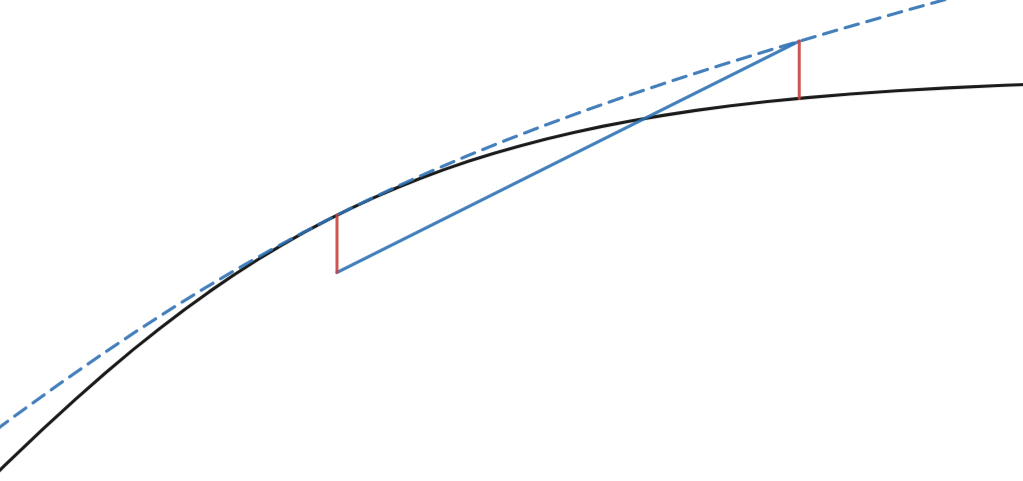
\includegraphics[width=5in]{figures/f-and-g.png}
		\caption{$f(x)$ (black) and a $g_i(x)$ (blue dashed)}
		\label{fig:f(x) with g(x)}
	\end{figure}
	And we can make another function $G(x)$ defined as 
	\[G(x) = \min_i(g_i(x))\]
	\subsection{Lemma}
	$\max(G(x) - f(x))$ is a lower bound to $\max(|f(x) - \bar{f}(x)|)$.\\
	
	Let $x_G$ be the value satisfying
	\[G(x_G) - f(x_G) = \max(G(x) - f(x))\]
	Assume we have $\bar{f}(x_G) - f(x) < G(x_G) - f(x_G)$ (or simply $\bar{f}(x_G) < G(x_G)$). Say at $x_G$, $\bar{f}(x) = m_ix+b_i$. If $x_{di}$ lies within $x_{ci}$ to $x_{ci+1}$, then by the definition of $G(x)$,
	\[f(x_{di}) - m_ix_{di}+b_i > G(x_G) - f(x_G)\].
	If $x_{di}$ lies outside $x_{ci}$ to $x_{ci+1}$, we can see that
	\[f(x) - \bar{f}(x) > f(x_{di}) - m_ix_{di}+b_i > G(x_G) - f(x_G)\]
	(This is hard to explain in words, but easy to see from a graph. We rely on $\bar{f}$ being continuous.)
	\begin{figure}[H]
		\centering
		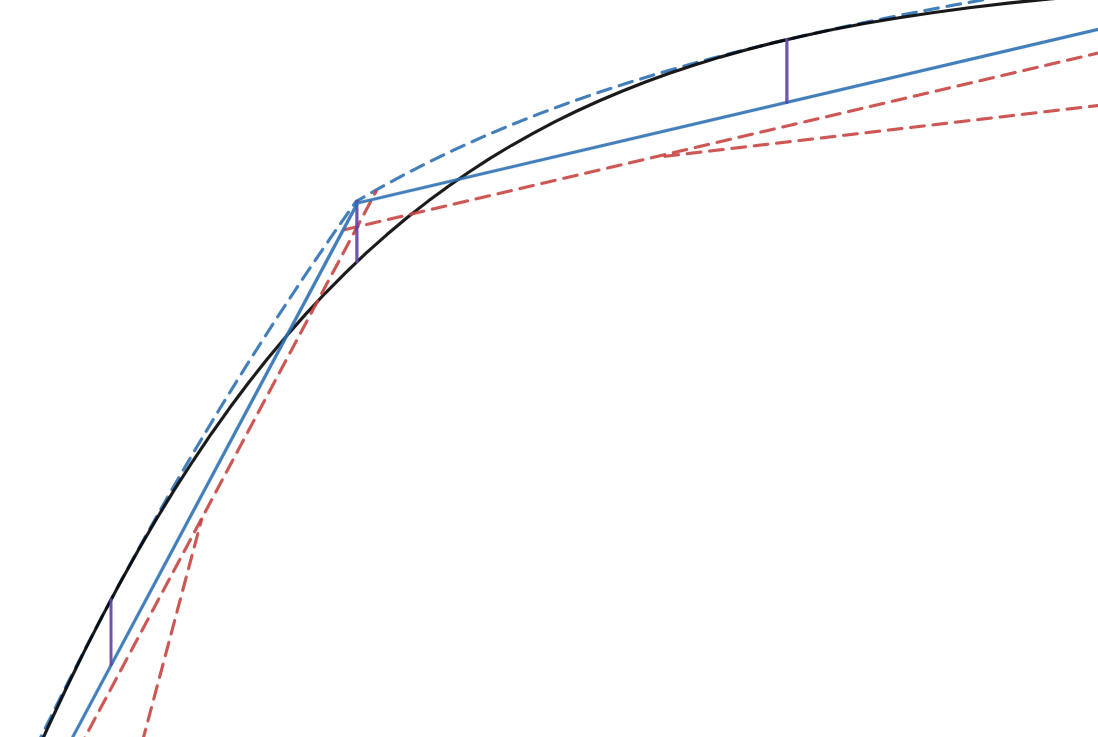
\includegraphics[width=4in]{figures/big-G-figure.png}
		\caption{This cluttered diagram (not to scale) explains this argument. In blue we have what I am proposing as the best PWL function. We can see that at three different places it has a variation $\Delta$ (purple lines). If we try to propose any other PWL with a smaller variation at $x_G$ (dashed red lines), this function must have a greater variation at one of the two $x_d$. If the function has another piecewise segment before reaching $x_d$ (branches on the dashed red lines), it will have a strictly greater variation.}
		\label{fig:G(x) and explanation of argument}
	\end{figure}
	\subsection{Final Steps}
	So we have that $\max(G(x) - f(x))$ is a lower bound to the maximum variation. Let's name this $\Delta$. If we can create a PWL function which has a maximum variation of $\Delta$ then we are done. This can be done by choosing starting at $x_G$ and expanding on either side, choosing the next $x_{c}$ when $m_ix+b_i$ intersects $G(x)$. To the left, this will eventually hit the x-intercept. To the right, this can repeat until we choose to round off to the asymptote. One thing I want to include in the tables in Results is how many line segments are required so that this round off is less than $\Delta$. 
	
	We can calculate $x_G$. We know $x_G$ will occur at a point where two $g(x)$ functions intersect, say $g_i(x)$ and $g_{i+1}(x)$. Then we can show that.
	\[x_G=\frac{f(x_{di}) - f(x_{di+1}) - m_ix_{d_i} + m_{i+1}x_{di+1}}{m_{i+1} - m_{i}}\]
	\[\Delta = g_i(x_G) - f(x_G)\]
	This means we can get a closed form solution if $x_{di}$ can be explicitly solved for. Otherwise we need the use of a numerical solver.
	
	\section{Results}
	I want to create tables for $x_c$ and $b$, also some graphs. Right now my code doesn't necessarily produce a continuous PWL function.
	
	\begin{center}
		\begin{tabular}{|c c|} 
			\hline
			f(x) & $\Delta$ \\
			\hline\hline
			$\sigma$ & 0.01132\\
			\hline
			$\arctan$ & 0.02606 \\
			\hline
			$\tanh$ & 0.02265 \\
			\hline
		\end{tabular}
	\end{center}
	\section*{Acknowledgments}
	

	
	\FloatBarrier
	\bibliography{references}
	
\end{document} 